%Tech Science Press — CMC variant of the MA-SQLGrid manuscript
%=================================================================
\documentclass[cmc,article,submit,moreauthors,pdftex]{Definitions/tsp}
\input{Definitions/package}
\input{Definitions/unicode}

\usepackage[OT1,OT2,T2A,T2B,T2C,T3,T5,T1]{fontenc}
\usepackage[russian,english]{babel}

%=================================================================
% Internal commands: Article information and pagination will be assigned by the Editorial Office
\continuouspages{}
\firstpage{1}
\makeatletter
\setcounter{page}{\@firstpage}
\makeatother
\pubvolume{0}
\issuenum{0}
\elocationid{0}
\articlenumber{0}
\pubyear{2026}
\copyrightyear{2026}
\datereceived{Day Month Year}
\dateaccepted{Day Month Year}
\dateonlinefirst{}
\datepublished{Day Month Year}

%=================================================================
% Full title of the paper (Capitalized)
\Title{MA-SQLGrid: A Multi-Stage Context-Grounding Framework for Text-to-SQL over Power Grid Maintenance Databases}

% Authors, for the paper (add full first names)
\Author{Bijing Liu\textsuperscript{1,2}, Chenglong Sun\textsuperscript{1,2} and Yong Yang\textsuperscript{1,2,*}}

% Authors, for metadata in PDF
\AuthorNames{Bijing Liu, Chenglong Sun and Yong Yang}

% Affiliations / Addresses
\address{%
\textsuperscript{1}NARI Group Corporation (State Grid Electric Power Research Institute), Nanjing 211106, Jiangsu Province, China

\textsuperscript{2}Beijing Kedong Electric Power Control System Co., Ltd., Beijing 100080, China
}%

% Contact information of the corresponding author
\corres{Corresponding Author: Yong Yang. Email: yangyong1@sgepri.sgcc.com.cn}

% Abstract (Do not use inserted blank lines, i.e. \\)
\abstract{Text-to-SQL for power-grid maintenance databases requires exact grounding to a fixed schema, canonical values, and an expected answer contract. This paper presents MA-SQLGrid, a lightweight multi-stage pipeline that selects compact schema/value context, normalizes domain expressions, infers answer shape, generates SQL, and applies reference-free execution-based validation. On the held-out 180-question split of the synthetic GridDB-Maintenance-v2 v0.1 benchmark, compact contract-aware context improves strict execution accuracy over full schema-values prompting from 0.4389 to 0.7000 with \texttt{gpt-5.4-mini} and from 0.3389 to 0.7000 with \texttt{deepseek-chat}. Validation raises the scores to 0.7278 and 0.7667, respectively; the original-generator increment is not statistically significant and is treated as diagnostic. Projection-tolerant rescoring reverses the compact-versus-full ordering for both generators, showing that the strict gain is dominated by projection and ordering conformance rather than superior row-content retrieval. Compact prompting reduces the rendered prompt estimate by 63.5\%; measured input tokens fall by 23.4\% on the original serving stack and 74.7\% on the direct second-model endpoint. Three temperature-0 repeats on the second generator show at most 1.1 percentage points of accuracy spread and 98.3\% per-question verdict agreement. A tenfold row-scaling diagnostic with two distractor tables preserves the strict compact-context advantage, but asymmetrically enlarges only the full-schema candidate space. The evidence supports the complete contract-aware pipeline on this single synthetic database. It does not independently identify compactness without a full $2\times2$ context-by-shape factorial, nor establish cross-database generalization.}

% List 3 to 10 pertinent keywords specific to the article
\keyword{Text-to-SQL; power grid maintenance databases; large language models; multi-stage prompting; schema linking; answer-shape inference; execution-based validation}

%%%%%%%%%%%%%%%%%%%%%%%%%%%%%%%%%%%%%%%%%%%
\begin{document}

\section{Introduction}\label{introduction}

Text-to-SQL remains fragile in domains where the database is fully known yet still difficult to verbalize precisely. Power-grid maintenance is a representative case: questions refer to equipment status, inspection outcomes, work orders, outage history, and date-bounded conditions, but the SQL answer depends on exact schema links and literal values. A user may say ``inactive transformer,'' ``latest inspection,'' or ``faulted feeder,'' while the database stores those concepts under specific column names and canonical values. This creates a recurring gap between natural language intent and executable SQL. The gap matters because the model can generate syntactically valid SQL that still returns the wrong denotation, especially when the question implies a particular answer shape such as a count, a grouped aggregate, a filtered list, or a scalar lookup. In a synthetic but deterministic maintenance database, the core challenge is therefore not open-ended reasoning. It is disciplined grounding against a fixed schema and value space \cite{zhong2020semantic,lei2020reexamining,liu2022semantic,quamar2022natural}.

Prior Text-to-SQL systems address pieces of this problem, but they tend to optimize one axis at the expense of another. Schema-linking methods improve token-to-column alignment, yet they still depend on the quality of the prompt context \cite{lei2020reexamining,gan2021robustness,liu2021awakening}. Prompt-based systems often help by adding demonstrations or structured cues, but full-schema prompting can inflate the context without solving literal mismatches \cite{chang2023prompt,nan2023enhancing,sun2023sqlprompt}. Decomposition and self-correction methods improve reasoning over joins and filters, yet their gains depend on how intermediate steps are grounded \cite{pourreza2023dinsql,wang2023macsql,talaei2024chess}. Recent surveys also point to a stable pattern: the strongest systems are not simply larger, but more selective about which schema evidence they expose and how they verify outputs \cite{liu2024survey,katsogiannismeimarakis2023survey,huang2024survey}. That observation motivates a narrower question for this benchmark: can compact domain context, not exhaustive schema exposure, improve a fixed generator on a frozen maintenance database?

MA-SQLGrid answers that question with a lightweight multi-stage design. A note on terminology: throughout this paper, MA-SQLGrid is described as a \emph{multi-stage} prompting pipeline with fixed, role-specialized stages (schema selection, value normalization, answer-shape inference, generation, and validation). It is not an interacting multi-agent system: the stages execute in a fixed order, do not negotiate or debate, and share no learned coordination policy. We retain the system name MA-SQLGrid for continuity with the released artifact package, but we deliberately avoid the term ``multi-agent'' for the architecture itself. The framework first builds compact schema/value context, then canonicalizes power-grid values, then infers the expected answer shape, and only then generates SQL with one fixed non-frontier model. A final validator compares candidate SQL using execution behavior, answer-shape consistency, and value alignment without gold SQL. This structure follows the spirit of CHESS-style context harnessing \cite{talaei2024chess} while remaining deliberately small enough to isolate the effect of grounding. The central idea is simple: in a narrow domain database, the generator should not see everything. It should see the few schema fragments and canonical values that most directly constrain the query, because those are the elements that determine whether the answer shape and the denotation are right \cite{wu2022chains,xie2022unifiedskg,li2024select}.

The main contributions of this paper are summarized as follows:
\begin{enumerate}[label=(\arabic*)]
\item It defines MA-SQLGrid, a compact multi-stage context-grounding framework for a deterministic power-grid maintenance database, with explicit schema selection, power-grid value normalization, and answer-shape inference in front of a single fixed generator.
\item It shows that the complete compact contract-aware condition outperforms schema-only and full-schema-values prompting under the same fixed generator (strict execution accuracy 0.7000 versus 0.4389), while explicitly separating this result from an unproven compactness-only mechanism because the study lacks a full $2\times2$ context-by-shape factorial.
\item It reports a reproducible evaluation protocol for GridDB-Maintenance-v2 v0.1, including the deterministic split, the evaluator contract, the comparator definitions, and an evaluation-convention sensitivity analysis that separates answer-contract conformance from row-content retrieval instead of taking the strict metric gap at face value \cite{zhong2020semantic,lee2021kaggledbqa,lei2024spider}.
\item It repeats the principal conditions with a second generator (\texttt{deepseek-chat}) under byte-identical prompts: the complete-pipeline gain (+36.1 points) and validation increment (+6.7 points) have the same direction, the convention-sensitivity finding replicates, and three temperature-0 repeats bound accuracy spread at 1.1 points with 98.3\% per-question verdict agreement. A deliberately bounded, asymmetric tenfold database-scale diagnostic records the associated accuracy and token behavior without claiming symmetric schema generalization.
\end{enumerate}

Where the paper speaks of robustness, the word is used in a bounded sense: robustness to schema/value and answer-shape ambiguity inside the fixed GridDB-Maintenance-v2 v0.1 protocol. The paper makes no claim of cross-benchmark robustness, production readiness, schema-drift tolerance, or stability across multiple random seeds. This distinction is important because the study is designed to isolate the effect of context construction and validation on one controlled benchmark, not to evaluate broad deployment behavior.

The rest of this paper is organized as follows. Section~2 reviews prompting, decomposition, and validation methods and positions this work against them. Section~3 formalizes the problem and presents the MA-SQLGrid framework. Section~4 describes the dataset, comparators, metrics, and experimental protocol. Section~5 reports and discusses the test-split results, including the convention-sensitivity analysis and the second-generator validation. Section~6 concludes and states the limitations.

\section{Related Work}\label{related-work}

\subsection{Text-to-SQL Prompting and Schema Grounding}\label{sect:rw1}

Prompt-based Text-to-SQL has shifted attention away from end-to-end training and toward how context is selected and structured \cite{chang2023prompt,nan2023enhancing,sun2023sqlprompt}. This line of work is effective because a fixed generator can be steered with schema summaries, demonstrations, or explicit instructions, but the result is highly sensitive to what is included. If the prompt is too broad, irrelevant tables and values compete for attention. If it is too narrow, the model loses the evidence needed for joins or predicates. Prior work on schema linking and grounded adaptation shows that local alignment between the question and the schema is a major determinant of executable SQL \cite{lei2020reexamining,liu2021awakening,liu2022semantic,gan2021robustness}. MA-SQLGrid follows this direction, but it treats compactness as a first-class design goal rather than a byproduct of retrieval.

Content-aware prompting has also demonstrated that database values matter when the question names concrete literals rather than only schema entities \cite{herzig2020tapas,chen2023large,zhang2024structure}. That lesson is especially relevant in maintenance databases, where status labels and categorical values frequently decide whether a candidate query is correct. Exhaustive schema dumping, however, is often a poor tradeoff in a fixed, narrow database because it adds many irrelevant tokens without improving the few literal matches that matter. MA-SQLGrid differs by selecting a compact subset of schema and values and by canonicalizing those values into a stable domain vocabulary before generation.

\subsection{Decomposition, Self-Correction, and Multi-Agent Orchestration}\label{sect:rw2}

Decomposition-based methods improve Text-to-SQL by breaking a query into smaller decisions before generating the final SQL \cite{liu2023divide,pourreza2023dinsql,arora2023adapt,xie2024decomposition}. Multi-agent systems extend that idea by assigning distinct roles for decomposition, generation, and refinement \cite{wang2023macsql,xie2024magsql,cen2025sqlfixagent}. These methods are attractive because they expose intermediate structure that can be checked against the question. Their drawback is overhead: each stage may reintroduce the same schema context, and the cost of multiple passes can outweigh the benefit when the database is simple and the schema is fixed.

MA-SQLGrid uses a similar role separation, but it is intentionally lighter. It does not rely on a large debate protocol or a broad search over many candidate generators. Instead, it uses compact schema/value context, answer-shape inference, and a single fixed generator, then validates the outputs with reference-free checks. This makes the method closer to CHESS-style context harnessing than to a search-heavy agent pipeline \cite{talaei2024chess,wang2023macsql,pourreza2023dinsql}. The difference matters because this benchmark rewards careful grounding more than open-ended reasoning depth, so a smaller control loop is enough to expose the main effect.

Schema pruning, execution-guided selection, and error-driven repair are individually established in the systems above. MA-SQLGrid tests a narrower combination---domain-targeted value canonicalization and explicit answer-shape inference in front of one fixed generator---on a frozen operational database rather than claiming broad cross-domain superiority.

\subsection{Execution-Based Evaluation and Validation}\label{sect:rw3}

Execution accuracy remains the most meaningful metric for Text-to-SQL because exact string match is too brittle to capture semantic equivalence \cite{zhong2020semantic,katsogiannismeimarakis2023survey,guo2023evaluating}. Execution-guided decoding and reranking use the database itself to reject malformed or inconsistent candidates \cite{wang2021executions,chen2023texttosql,li2024select}. More recent verification-oriented work extends this idea with semantic checks that do not require gold SQL at inference time \cite{huang2024survey,beyer2022verification,pauwels2024validation}. MA-SQLGrid adopts that principle in its final selection stage, but limits the validator to lightweight, reference-free checks so that the method remains compact and contract-compatible.

This distinction is important. Validation can improve selection, but it also adds latency and can become brittle if it overweights shape or execution signals. MA-SQLGrid therefore treats validation as a refinement layer, not the main source of performance. That framing differentiates it from methods whose primary contribution is broader search, self-correction, or execution-aware reinforcement \cite{wang2023macsql,zhai2025excot,pourreza2024chasesql}. The present work focuses on a narrower claim: when context is already compact and domain-grounded, reference-free validation can improve the final choice without requiring gold SQL.

Recent Text-to-SQL work also reinforces the need to position compact domain grounding separately from broad benchmark generalization. Retrieval and schema-simplification systems such as CORE-T and UNJOIN focus on selecting coherent schema evidence before generation \cite{soliman2026coret,ganesan2025unjoin}. Multi-agent or refinement systems such as MARS-SQL, SEA-SQL, and SIRIUS-SQL emphasize iterative candidate improvement or execution feedback \cite{yang2025marssql,li2024seasql,luo2026siriussql}. Evaluation-oriented work such as SpotIt+, SQLStructEval, and production SQL accuracy studies examine how to validate generated SQL beyond string match \cite{tremante2026spotit,zhou2026sqlstructeval,arif2026agentagnostic}. These very recent works are used as contemporary preprint context, not as settled archival baselines that define the claims of this paper. Closest to the present setting, Borov\v{c}ak et al.~\cite{borovcak2026evaluating} evaluated open-source LLM agents for SQL generation and structured analytics on relational databases in this journal, comparing model families and single-agent versus multi-agent architectures on business-analytics workloads and the Spider benchmark. MA-SQLGrid is complementary to that agent-evaluation perspective: instead of comparing generators and agent architectures, it fixes one generator and asks whether domain-grounded compact context construction and reference-free validation improve Text-to-SQL on a frozen operational power-grid database under an auditable local protocol. MA-SQLGrid intersects all of these themes, but its contribution is deliberately narrower: it tests whether a small, fixed-schema power-grid database benefits from compact schema/value grounding and reference-free validation.

\section{Method}\label{method}

\subsection{Problem Formulation}\label{sect:m1}

Let a natural-language question be $q$, and let the database schema be $S$, with tables, columns, keys, and types extracted from \texttt{schema.sql}. Let $V$ denote the available value hints drawn from the database contents and dataset annotations. The task is to generate SQL $y$ such that executing $y$ on the database $D$ yields the intended denotation $a$. We write the objective as
\begin{equation}
y^* = \arg\max_{y \in \mathcal{Y}} P(y \mid q, C(q,S,V)),
\end{equation}
where $C(\cdot)$ is a compact context constructor that selects schema and value evidence relevant to the question.

MA-SQLGrid decomposes $C$ into schema selection, value canonicalization, and answer-shape estimation. Schema selection identifies tables and columns likely to participate in the query. Value canonicalization maps domain expressions such as status labels, categories, and temporal forms to canonical database values. Answer-shape estimation predicts whether the query should return a scalar, grouped aggregate, set-valued list, or filtered record list. The generator then produces candidates conditioned on the compact context and the inferred shape. At inference time, no gold SQL is available, so selection must rely on the candidate SQL itself and the local database response.

\subsection{Framework Overview}\label{sect:m2}

MA-SQLGrid is designed around a narrow but useful objective: for a question $x$, a fixed schema $S$, and a database instance $D$, produce SQL that executes to the intended denotation. The system does not learn a new parser. Instead, it changes how the input to a fixed generator is assembled and how candidate outputs are chosen. That choice matches the structure of the benchmark. In a frozen maintenance database, many errors come from overexposed schema context, literal mismatch, or an incorrect answer shape, rather than from a lack of general language competence \cite{wu2022chains,talaei2024chess,pourreza2023dinsql}.

Formally, the framework constructs a compact context $c$ from $x$, $S$, and $V$ using three components: a selector $g$, a normalizer $n$, and a shape predictor $h$. The resulting context is
\begin{equation}
c = g(x,S,V) \oplus n(x,V) \oplus h(x),
\end{equation}
where $\oplus$ denotes concatenation into a prompt-ready representation. Given that context, the fixed generator produces a small set of candidate SQL strings,
\begin{equation}
\{y_1,\dots,y_k\} \sim p_\theta(y \mid x,c),
\end{equation}
and the validator assigns each candidate a score that combines execution success, answer-shape consistency, value alignment, and a small complexity penalty:
\begin{equation}
s(y_i; x,c,D) = \lambda_1 \mathrm{Exec}(y_i,D) + \lambda_2 \mathrm{Shape}(y_i,h(x)) + \lambda_3 \mathrm{Value}(y_i,n(x,V)) - \lambda_4 \mathrm{Cost}(y_i).
\end{equation}
The final prediction is the highest-scoring executable candidate. This objective is reference-free at inference time and depends only on the candidate SQL, the compact context, and the database behavior \cite{zhong2020semantic,beyer2022verification,huang2024survey}. Fig.~\ref{fig:architecture} summarizes the architecture, and the rest of the implementation follows a fixed schedule: question analysis, domain normalization, compact prompt assembly, generation, execution, and selection. The method is therefore best understood as a controlled multi-stage prompting system rather than a search-heavy agent loop. It is lightweight by design, but each stage removes a specific failure mode that the benchmark makes visible.

\begin{figure}[H]
\centering

\includegraphics[width=11.9cm]{charts/architecture_diagram_1.png}
\caption{MA-SQLGrid architecture: fixed multi-stage schedule from question analysis through compact context construction, generation, and reference-free validation.}
\label{fig:architecture}
\end{figure}

\subsection{Compact Schema/Value Selection}\label{sect:m3}

The first component is compact schema/value selection. The component ablation of Section~5 attributes the largest single share of the end-to-end gain to the answer-shape channel that this compact context carries (removing shape hints drops correct answers from 126 to 77), with the schema/value reduction itself contributing through disambiguation and attention economy rather than dominating the gain on its own. MA-SQLGrid does not expose the full schema. It scores schema items by lexical overlap with the question, relation proximity, and domain salience, then keeps only the subset needed to express the likely joins and predicates. In the implementation used for the formal run, lexical matching is applied to table names, column names, and value mentions; selected tables are expanded through foreign-key neighbors up to a fixed cap; and the domain selector prioritizes maintenance-relevant entities such as assets, work orders, sensor readings, and topology edges when the question contains corresponding operational phrases. The same reduction applies to values: only the hints that help disambiguate maintenance categories, status labels, and temporal forms are retained. This is not a compression trick for its own sake. In a narrow database, irrelevant schema tokens do not improve coverage; they dilute attention. The test results support that choice: the compact-domain condition reaches 0.7 execution accuracy while using far fewer estimated prompt tokens than the full-schema baseline. That pattern is consistent with selective grounding work in schema linking and structured retrieval \cite{lei2020reexamining,lin2020bridging,quamar2022natural,xie2022unifiedskg}.

\subsection{Power-Grid Value Normalization}\label{sect:m4}

The second component, power-grid value normalization, maps question phrasing into canonical database literals before generation. The normalizer is a fixed domain dictionary and pattern set over the local value inventory, not a learned classifier and not a lookup into gold SQL. If the question uses an abbreviated or colloquial form, the normalizer resolves it to the local database value that the SQL must contain. If the question mentions a status or asset class, the system converts that mention into the dataset's canonical vocabulary. For example, phrases such as ``offline assets,'' ``closed topology connection,'' and ``temperature alarm'' are converted into candidate predicates over the corresponding status, topology, or sensor columns. The local inventory used by the formal run contains 196 distinct values across 28 non-ID categorical, date, status, flag, and text columns; on the 180-question test split, the domain context emitted at least one normalized value hint for 170 questions, with 330 hint instances and 111 unique rendered hints. This matters because the benchmark is deterministic: value mismatches are not random noise but predictable lexical failures. Separating normalization from generation makes the generator's task smaller and more stable. It also explains why MA-SQLGrid improves on schema-only and full-schema-values prompting: the prompt is not merely shorter or longer, it is aligned with the database's literal conventions \cite{brunner2020valuenet,chen2023large,liu2022semantic}.

\subsection{Answer-Shape Inference}\label{sect:m5}

The third component, answer-shape inference, predicts the form of the answer before SQL is generated. Let $\mathcal{T}$ be a small set of shape classes such as scalar, grouped aggregate, set-valued list, filtered record list, and boolean. The predictor computes
\begin{equation}
h(x) = \arg\max_{t \in \mathcal{T}} p_\phi(t \mid x),
\end{equation}
where $\phi$ is a prompt-derived policy inside the framework. The purpose is to constrain the candidate space, not to solve semantics independently. Questions that ask ``how many,'' ``which,'' ``whether,'' or ``latest'' tend to require different SQL skeletons, and the wrong skeleton often yields a valid but semantically wrong query. Injecting shape into the context gives the generator an inexpensive structural prior. That is why the generic CHESS-style baseline improves shape accuracy relative to schema-only prompting, but the domain-grounded version improves much more once shape is coupled with canonical value hints \cite{liu2023divide,talaei2024chess,wang2023macsql}.

\subsection{Generation, Reference-Free Validation, and Bounded Repair}\label{sect:m6}

The generator stage uses one fixed non-frontier model, \texttt{gpt-5.4-mini}, with deterministic decoding at temperature 0; a second-generator replication with \texttt{deepseek-chat} under byte-identical prompts is described in Section~4. Fixing the model isolates the framework effect from any effect of a stronger generator family. The model receives the compact schema/value context, the normalized domain hints, and the answer-shape cue, then returns candidate SQL in a controlled format. Deterministic decoding is useful here because it turns the comparison into a question of context and validation, not sampling variance. Exact future reproducibility can still be affected by hosted-model drift, so the artifact package retains the model identifier, prompts, context hashes, raw outputs, selected SQL, retries, token estimates, and serving logs needed to audit the reported run \cite{chang2023prompt,nan2023enhancing,sun2023sqlprompt}.

The final stage is reference-free execution, shape, and value validation. Each candidate is executed on the local SQLite database. Candidates that fail syntax or execution are discarded. Among executable candidates, the validator checks whether the observed result shape matches the inferred answer shape and whether the SQL predicates align with the normalized value hints. The selected query is the one with the highest composite score. The cost is linear in the number of candidates, so the validation layer increases latency, but it also explains the measured improvement in answer-shape accuracy and final execution accuracy \cite{wang2021executions,li2024select,huang2024survey}.

The ranking policy is conservative by design. Executable candidates outrank non-executable ones; among executable candidates, shape-consistent queries outrank shape-inconsistent ones; and among those, candidates with stronger value alignment and lower syntactic complexity are preferred. The implementation uses fixed integer weights for these checks: safety and execution success receive the largest positive weights, shape agreement and ordering agreement receive smaller positive weights, empty results and missing value hints are penalized, matched value hints add reward, and candidate order is used as a deterministic tie-breaker. These weights are fixed before reporting and are not tuned on the test split. The system never requires gold SQL, gold answers, or hand-coded rules for specific labels. Its signal comes from the candidate SQL and the database response. That aligns the validator with the same execution contract used in the experiments, which is essential for a paper focused on validated denotation rather than string matching.

For reproducibility, the C5 condition fixes the candidate and repair policy rather than leaving it to an open-ended agent loop. C5 generates at most five candidate SQL strings from the same compact domain context used by C4. Each candidate is checked by the local read-only SQL guard before execution. The ranking signal combines four reference-free checks: whether execution succeeds, whether the observed result shape is compatible with the inferred answer shape, whether the SQL preserves the inferred value hints, and whether ordering cues are respected when the question implies an ordered or top-k answer. If two candidates receive the same effective validation status, the earlier generated candidate is preferred, which gives deterministic tie-breaking under temperature-zero decoding.

The repair boundary is also fixed. C5 permits one repair opportunity when the initially selected candidate fails execution, violates the inferred shape, misses inferred value hints, or ignores an inferred ordering cue. The repair prompt receives the original question, the compact context, the failed SQL, and the reference-free validation signal. It does not receive gold SQL, gold denotation rows, evaluator correctness, required-literal metadata, answer-shape metadata, or order-sensitive metadata. A repaired SQL string is accepted only if it executes and does not worsen the available reference-free validation signal. If no candidate can be extracted, the runner records an error and emits a safe placeholder rather than silently fabricating a successful query. The archived formal run reported zero contract errors, zero unsafe SQL records, zero provider/extraction errors, and zero leakage-scan problems. Thus, the validation layer is reproducible as a bounded selector over generated candidates, not as an unconstrained self-correction process. The full set of implementation details fixed in the reported run, including the schema-selection rules, the C5 ranker weights, and the no-gold prediction contract, is provided in Table~S1 of the Supplementary Materials.

\section{Experimental Setup}\label{experiments}

\subsection{Dataset and Database}\label{sect:e1}

The evaluation uses only the verified local dataset GridDB-Maintenance-v2 v0.1, with the schema, SQLite database, question file, split file, annotation protocol, and verification log retained in the artifact package. It contains 200 question-SQL pairs and follows a deterministic split: Q001--Q020 are dev and Q021--Q200 are test. The dev split is reserved for feasibility checks and prompt calibration, while the formal comparison uses the held-out 180-question test split. That split discipline is central to the paper because the dataset is small, frozen, and deterministic, so leakage would be easy to miss but would distort every downstream claim.

The database contains eight tables covering asset types, assets, grid topology, locations, maintenance logs, sensor readings, technicians, and work orders. The schema is compact but relationally connected. The largest entity table is \texttt{assets} with 18 rows and seven columns for asset identity, type, location, installation date, status, and capacity. The work-order table contains 15 rows and covers priorities, statuses, scheduled and completed dates, assigned technicians, and fault codes. The sensor table contains 26 readings with sensor type, value, unit, timestamp, and alarm flag. Supporting tables provide six asset types, eight locations, eight technicians, eight maintenance logs, and nine topology edges. This structure creates a useful test bed for schema/value grounding because many questions require joins from assets to asset types, locations, work orders, readings, or topology relations.

The value space is small enough to enumerate but rich enough to create literal-binding failures. Asset types are \texttt{Breaker}, \texttt{Capacitor}, \texttt{Line}, \texttt{Relay}, \texttt{Substation}, and \texttt{Transformer}; voltage classes are \texttt{33kV}, \texttt{115kV}, and \texttt{230kV}; asset statuses are \texttt{in\_service}, \texttt{maintenance}, and \texttt{offline}; location regions are \texttt{Central}, \texttt{East}, \texttt{North}, \texttt{South}, and \texttt{West}; work-order statuses are \texttt{completed}, \texttt{open}, and \texttt{scheduled}; priorities are \texttt{high}, \texttt{medium}, and \texttt{low}; and fault codes include \texttt{BREAKER}, \texttt{CAP}, \texttt{INSPECT}, \texttt{LINE}, \texttt{LOAD}, \texttt{RELAY}, \texttt{SUB}, \texttt{TEMP}, and \texttt{VOLT}. Other important vocabularies include technician specialties, sensor types (\texttt{load}, \texttt{power\_factor}, \texttt{temperature}, \texttt{voltage}), sensor units (\texttt{C}, \texttt{MW}, \texttt{kV}, \texttt{pu}), topology connection types (\texttt{control}, \texttt{feeder}, \texttt{tie}), and switch states (\texttt{closed}, \texttt{open}). These values explain why exhaustive schema exposure is not enough: the correct SQL often depends on mapping a natural-language phrase to one of a few exact local literals.

The question annotations also show why answer-shape control is central. Among the 200 questions, 187 include a filter tag, 131 include an order-by tag, 113 require a join, 66 involve aggregation, 33 include a time predicate, 20 involve top-k selection, 16 use group-by, 12 involve topology traversal, and 10 require a self-join. The difficulty labels are 74 easy, 102 medium, and 24 hard. The most frequently referenced table is assets with 120 question annotations, followed by work orders with 72, locations with 54, asset types with 40, sensor readings with 31, technicians with 19, grid topology with 12, and maintenance logs with 7. This distribution makes the benchmark a focused test of join selection, literal normalization, ordering, and result-shape control rather than a generic SQL stress test. A tabular dataset characterization is provided in Table~S2 of the Supplementary Materials.

\subsection{Conditions and Generators}\label{sect:e2}

The formal comparison centers on five short condition labels, C1 through C5, chosen to isolate the effect of compact grounding and validation. C1 is a schema-only direct prompt. C2 exposes the full schema and values in a direct prompt. C3 is a CHESS-inspired generic multi-stage prompt without power-grid-specific normalization and shape discipline; it is a prompt baseline motivated by CHESS, not a reproduction of the complete CHESS system. C4 is the proposed compact domain-grounded method. C5 adds reference-free validation and candidate ranking. The verbatim templates for all five conditions are reproduced in Section~S1 of the Supplementary Materials.

The main generator is a fixed \texttt{gpt-5.4-mini} configuration with \texttt{temperature=0}. Fixing the model matters because it removes generator-family variation from the comparison. The paper is therefore not a study of model scaling. It is a study of how context construction and validation change the behavior of one fixed generator on a narrow deterministic database. The exact serving logs, prompts, context hashes, model identifier, retries, token estimates, predictions, and scores are retained with the artifact package for reproducibility.

To test whether the reported effects are specific to one generator family, the study adds a second-generator protocol. The C2, C4, and C5 conditions were re-run with \texttt{deepseek-chat}, accessed through the provider's direct OpenAI-compatible endpoint (\texttt{api.deepseek.com/v1}) at temperature 0, on the same 180 held-out test questions. The second-model runner reuses the archived formal-run prompts byte-for-byte, so both generators receive identical inputs for C2 and C4 and identical candidate-generation prompts for C5. The C5 validation, ranking, and repair stage, whose original implementation is tied to the archived pipeline, was reimplemented from the specification in Section~3 (identical guard, ranker weights, and bounded-repair policy) and validated against the archive before use: on the archived \texttt{gpt-5.4-mini} candidate sets it reproduces 167 of 169 non-repair selection decisions (98.8\% agreement). Scoring uses the same packaged evaluator under the same strict contract. The second-generator run comprised 540 calls with zero provider errors and a safe-SQL rate of 1.0 in all three conditions. A companion consistency check repeated C4 and C5 three times each at temperature 0 on the same generator (1,080 additional calls) to bound run-to-run variation. Both are reported in Section~\ref{second-generator-validation}.

The intended release package contains the dataset files, schema, SQLite database, split file, annotation protocol, evaluator, condition prompts, context hashes, prediction and score records, trace files, component-ablation addendum outputs, validator diagnostics, final \LaTeX/PDF sources, and citation-verification artifacts. This release boundary is important because the paper's claims are local to the fixed artifact package rather than to a mutable hosted endpoint or an unreported private benchmark.

Each test question is converted into a condition-specific prompt, sent to the fixed generator, optionally passed through reference-free validation, executed against \texttt{database.sqlite}, and scored by the same local semantic evaluator. Only context construction and validation differ across the ablations.

\subsection{Metrics, Prediction Contract, and Evaluation Conventions}\label{sect:e3}

The primary metric is execution accuracy by validated denotation, computed with the local semantic evaluator in \texttt{evaluator/evaluator.py}. If $N$ is the number of test questions and $z_i \in \{0,1\}$ indicates whether the predicted SQL for question $i$ matches the validated denotation, then execution accuracy is
\begin{equation}
\mathrm{Acc} = \frac{1}{N}\sum_{i=1}^{N} z_i.
\end{equation}
Higher is better, and the value lies in $[0,1]$. Secondary metrics include safe-SQL rate, executable-SQL rate, answer-shape accuracy, prompt token estimate, latency, provider failure rate, and unsafe-SQL rate. Safe-SQL rate measures whether the prediction passes the read-only SQL guard. Executable-SQL rate measures whether the guarded query actually executes on \texttt{database.sqlite}. These two rates are reported separately because a query can be safe and still fail at execution time, for example by using a nonexistent column. Answer-shape accuracy measures agreement between the predicted result shape and the inferred or annotated shape. Prompt token estimate tracks input size. Latency measures end-to-end runtime per question. Provider failure rate and unsafe-SQL rate are reported because they distinguish model instability from benchmark difficulty.

All SQL generation ran through the hosted model API; the local machine only assembles prompts, executes SQLite queries, and scores results, so no local GPU is involved in any reported number. All five conditions achieved a safe-SQL rate of 1.0, with no provider failures and no unsafe SQL. Executable-SQL rates were 1.0000 for C1 and C2, 0.9167 for C3, 0.8889 for C4, and 0.9722 for C5. These numbers matter because they separate safety and availability from semantic correctness. The main variation is therefore whether the framework selects an executable query with the right denotation and answer shape.

The experiment uses a fixed prediction contract so that the comparison is auditable. Each record stores the condition, prompt/context hashes, selected SQL, candidate list, selected-candidate index, trace path, latency, token estimates, retry count, and error field. It excludes gold SQL, gold result rows, evaluator correctness labels, expected result hashes, required-literal metadata, answer-shape metadata, and order-sensitive metadata. Those excluded fields are used only after prediction generation for scoring and diagnostics. Likewise, the held-out audits, residual-error tables, and illustrative examples in this paper are post-generation diagnostics; they did not feed the prompts, normalizer rules, ranker weights, repair prompts, or candidate-selection decisions. This boundary is essential because C4 and C5 depend on inferred shape and inferred value hints; using dataset metadata in prompts or rankers would no longer test the proposed mechanism. The formal run produced 900 predictions and 900 score records, corresponding to 180 test questions times five conditions under the deterministic seed label, with zero contract errors, zero unsafe SQL records, zero provider or extraction errors, and zero leakage-scan problems.

Two evaluation conventions inherited from the dataset annotation protocol must be stated explicitly, because they interact with the proposed method. First, every multi-row gold query carries a deterministic \texttt{ORDER BY} clause, and 131 of the 200 questions are annotated order-sensitive, so the strict evaluator compares row sequences for those questions. Second, every gold query projects exactly the minimal column set recorded in the annotation's answer-shape metadata, and the strict evaluator rejects any prediction whose column count differs. The answer-shape inference stage of MA-SQLGrid encodes precisely these two conventions as question-derived hints (expected projection count, row granularity, and a deterministic-ordering flag). All five conditions receive the same instruction text asking the model to match the requested projection and use deterministic ordering, but only C4 and C5 receive the inferred hints that make the conventions explicit for the specific question; C1--C3 must recover them from the question wording alone. Part of the headline gap between C4/C5 and the baselines is therefore attributable to convention conformance rather than to row-content grounding. Section~\ref{evaluation-convention-sensitivity} quantifies this dependence directly by reporting two auxiliary relaxed metrics alongside the strict metric, so the reader can separate the two effects instead of taking the strict gap at face value.

The single-pass protocol should be interpreted carefully. The formal seed value is a reproducibility label for the deterministic evaluation, not a random-seed sample from which run-level variance can be estimated. Two pieces of trace-level determinism evidence bound the protocol risk: decoding temperature was fixed at 0 for every call, and of the 900 archived API calls, 898 succeeded on the first attempt while 2 (one in C1, one in C4) required a single retry; the final records contain no provider errors. This documents that the reported single pass was not silently stabilized by repeated sampling, but it does not replace a repeated-run consistency study; such a study is provided for the second generator in Section~\ref{second-generator-validation}. The paired sign tests compare per-question binary outcomes within the fixed 180-item test set, so they are useful for showing how often one condition answers a question correctly when another condition does not. They do not establish multi-run stability.

\section{Results and Discussion}\label{results}

\subsection{Main Results}\label{sect:r1}

Table~\ref{tab:main-results} reports the formal protocol summary on the held-out test split.

\begin{table}[H]
\tablesize{\small}
\caption{Formal protocol summary for the held-out GridDB-Maintenance-v2 v0.1 test split (180 questions, fixed \texttt{gpt-5.4-mini} generator, temperature 0). Best execution accuracy in bold.}
\label{tab:main-results}
\centering
\begin{adjustbox}{max width=\textwidth}
\begin{tabular}{llrrrr}
\toprule
\textbf{Condition} & \textbf{Role} & \textbf{Prompt tokens} & \textbf{Latency ms} & \textbf{Executable SQL} & \textbf{Execution accuracy} \\
\midrule
C1 & Schema-only direct generation & 381.3 & 3259.8 & 1.0000 & 0.3944 \\
C2 & Full schema and values direct generation & 710.3 & 2959.0 & 1.0000 & 0.4389 \\
C3 & CHESS-inspired prompt baseline & 202.0 & 2895.1 & 0.9167 & 0.4000 \\
C4 & Compact domain context & 259.2 & 2887.5 & 0.8889 & 0.7000 \\
C5 & Compact context with validation & 258.2 & 5562.5 & 0.9722 & \textbf{0.7278} \\
\bottomrule
\end{tabular}
\end{adjustbox}
\end{table}

Table~\ref{tab:main-results} captures the core resource tradeoff. The estimated prompt-token column measures the condition-specific context template rendered by the experiment runner: the full-schema context is almost three times the size of the compact-domain context (710.3 versus 259.2 estimated tokens, a 63.5\% reduction), yet it performs substantially worse. The validation condition keeps the prompt nearly as small as the unvalidated compact variant, but its latency rises because it scores multiple candidates. The gain is not free, but it is also not purchased by simply exposing more context.

\begin{table}[H]
\tablesize{\small}
\caption{Measured API resource consumption per question, aggregated from the 900 archived provider-reported usage records (180 questions per condition). Input/output tokens are the provider's counts, which include serving-side overhead shared by all conditions; C5 combines candidate generation and, when triggered, one repair call.}
\label{tab:real-tokens}
\centering
\begin{adjustbox}{max width=\textwidth}
\begin{tabular}{lrrrrr}
\toprule
\textbf{Condition} & \textbf{Input tokens (mean)} & \textbf{Output tokens (mean)} & \textbf{Latency ms (mean)} & \textbf{Latency ms (median)} & \textbf{First-attempt calls} \\
\midrule
C1 & 5007.7 & 45.0 & 3259.8 & 1998.0 & 179/180 \\
C2 & 6346.7 & 45.8 & 2959.0 & 1999.5 & 180/180 \\
C3 & 4756.3 & 47.3 & 2895.1 & 1959.0 & 180/180 \\
C4 & 4859.0 & 52.0 & 2887.5 & 2102.5 & 179/180 \\
C5 & 5309.8 & 197.5 & 5562.5 & 3845.5 & 180/180 \\
\bottomrule
\end{tabular}
\end{adjustbox}
\end{table}

Table~\ref{tab:real-tokens} complements the estimated column with the provider-reported token usage of the actual run, and the two views must not be conflated. The measured input cost of C4 is 4859.0 tokens per question against 6346.7 for C2, a 23.4\% reduction, far smaller than the 63.5\% template-level reduction. The difference is a fixed serving-side overhead of roughly 4500--4600 input tokens per call that is identical across conditions (visible in C1, whose template is only 381.3 estimated tokens but whose measured input is 5007.7). The honest efficiency statement is therefore: compact grounding shrinks the controllable part of the prompt by about a factor of 2.7, which translated into a 23.4\% end-to-end input-token saving under this serving stack; deployments with less fixed overhead would realize proportionally more. The second-generator run (Section~\ref{second-generator-validation}) confirms this reading on a clean endpoint: on \texttt{deepseek-chat}, served directly by its provider with negligible fixed overhead, the same C4-versus-C2 contrast yields a measured 74.7\% input-token reduction (509.3 versus 2011.6 tokens per question). The three numbers triangulate consistently: the template-level estimate (63.5\%) sits between the overhead-masked measurement on the original stack (23.4\%) and the near-overhead-free direct measurement (74.7\%), so the direct endpoint corroborates, rather than contradicts, the template estimate. On the output side, C5 consumes about four times the completion tokens of C4 (197.5 versus 52.0 per question) because it requests multiple candidates and occasionally a repair, which is the direct cost of the validation layer. The complete formal run consumed 4.73M input tokens and 69.8k output tokens across the 900 calls.

The formal results were obtained in one deterministic pass over the test split, so the reported values are single-run outcomes rather than averages over repeated seeds. The paired comparisons (Supplementary Table~S3) show that C4 is correct on 49 questions that C2 misses, while the reverse holds for only 2 questions (mean difference +0.2611, exact sign test $p = 1.179\times10^{-12}$); C5 versus C2 shows 56 versus 4 such questions (+0.2889, $p = 9.085\times10^{-13}$). By contrast, C5 versus C4 is 12 versus 7 (+0.0278, $p = 0.3593$). Thus, the compact condition changes strict contract-compliant success reliably, whereas the additional validation layer provides only a nonsignificant numerical increment in the original run and is not claimed as a confirmed standalone gain.

Fig.~\ref{fig:main-results} visualizes the execution-accuracy gap across conditions. C4 captures the principal grounding gain without added latency, whereas C5 incurs multi-candidate validation cost for a smaller additional gain. The Wilson intervals are item-level intervals over test questions, not confidence intervals over repeated model runs.

\begin{figure}[H]
\centering
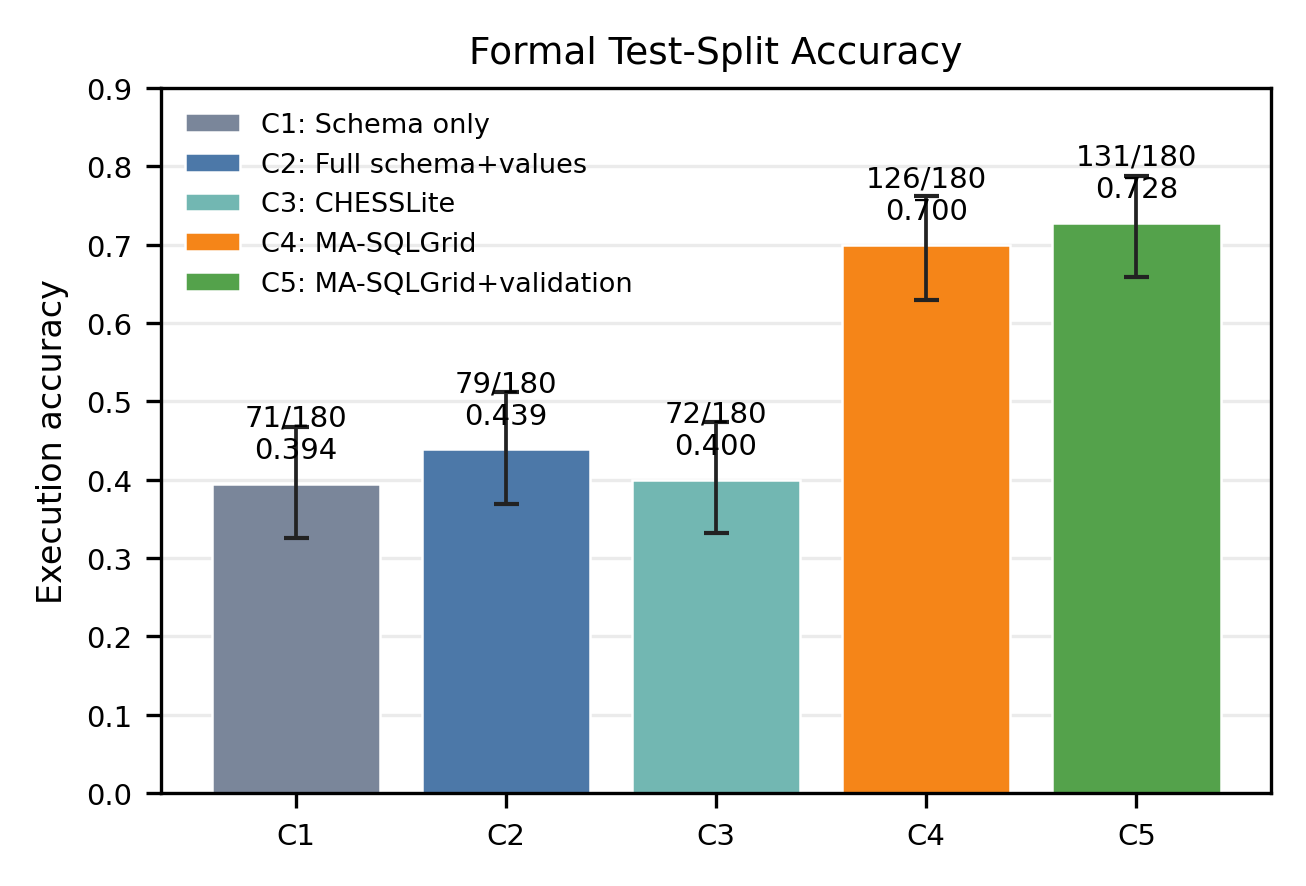
\includegraphics[width=11cm]{charts/fig_main_results.png}
\caption{Formal test-split execution accuracy by condition with item-level Wilson intervals over the 180 test questions.}
\label{fig:main-results}
\end{figure}

The answer-shape metric adds a second layer of interpretation. C1 reaches answer-shape accuracy of 0.3278, C2 reaches 0.3667, C3 reaches 0.5056, C4 reaches 0.8889, and C5 reaches 0.9722. The shape gain from C3 to C4 is substantial, which suggests that generic multi-stage prompting is not enough on its own. Shape inference matters most when it is paired with domain normalization. The validated condition then improves shape consistency again, which indicates that validation is not only rejecting invalid SQL but also preferring candidates whose result form matches the question.

Value-hint coverage is treated as an internal trace diagnostic rather than a headline metric: in the runner, a prediction with no inferred value hints receives a vacuous coverage value of 1.0, so this quantity is useful for auditing domain-context traces but not for ranking conditions. The stronger evidence for value grounding is instead the paired accuracy gap between C4 and C2. The trace-level coverage audit helps interpret this point without changing the main metric: among the 180 held-out test questions, 170 produced at least one normalized value hint in the domain context, with 330 normalized hint instances and 111 unique rendered hints over 20 matched value columns. These numbers are not used to score predictions, but they show that the normalizer was active on most of the formal split rather than only on a small hand-picked subset.

\subsection{Evaluation-Convention Sensitivity}\label{evaluation-convention-sensitivity}

All 900 predictions were also re-scored with order-insensitive and projection-tolerant variants. Relaxing order alone preserves the condition ranking, but projection tolerance raises C2 from 0.4389 to 0.8722, above C4 at 0.7444; C4 itself gains nothing from projection tolerance. Thus, the large strict advantage is dominated by answer-contract conformance---minimal projection and deterministic ordering---rather than superior row-content retrieval. The strict metric remains operationally relevant, but the relaxed result bounds the claim: compact grounding improves contract-compliant answers on this benchmark, not the baseline's ability to locate rows. Table~\ref{tab:second-model} reports the corresponding strict and relaxed values for both generators and shows that the reversal replicates on \texttt{deepseek-chat}.

\subsection{Component Ablation}\label{sect:r3}

To separate the two prompt-side components more directly, an addendum run removed one C4 hint channel at a time while preserving the same held-out test split, generator, temperature-zero decoding, and no-gold prediction contract. The addendum does not replace the formal C1--C5 comparison, but it clarifies the mechanism. Removing value hints reduces C4 from 126/180 to 118/180 correct. Removing answer-shape hints reduces it to 77/180 correct and lowers answer-shape accuracy to 0.4389. The result supports a bounded component-level interpretation: value normalization contributes a measurable additional gain, while answer-shape hints are a central part of the compact-context effect on this benchmark.

\subsection{Second-Generator Validation and Consistency}\label{second-generator-validation}

The second-generator protocol described in Section~4 re-ran C2, C4, and C5 with \texttt{deepseek-chat} on the same 180 held-out test questions using byte-identical archived prompts and the same packaged evaluator. Table~\ref{tab:second-model} reports strict and relaxed metrics for both generators side by side.

\begin{table}[H]
\tablesize{\small}
\caption{Cross-model comparison on the 180-question test split under strict and relaxed metrics. The \texttt{deepseek-chat} rows use byte-identical prompts, temperature 0, and the same evaluator.}
\label{tab:second-model}
\centering
\begin{adjustbox}{max width=\textwidth}
\begin{tabular}{llrrr}
\toprule
\textbf{Generator} & \textbf{Condition} & \textbf{Strict (primary)} & \textbf{Order-insensitive} & \textbf{Order-insensitive + projection-tolerant} \\
\midrule
\texttt{gpt-5.4-mini} & C2 & 0.4389 (79/180) & 0.4778 & 0.8722 \\
\texttt{gpt-5.4-mini} & C4 & 0.7000 (126/180) & 0.7444 & 0.7444 \\
\texttt{gpt-5.4-mini} & C5 & 0.7278 (131/180) & 0.7722 & 0.8056 \\
\midrule
\texttt{deepseek-chat} & C2 & 0.3389 (61/180) & 0.3667 & 0.8500 \\
\texttt{deepseek-chat} & C4 & 0.7000 (126/180) & 0.7944 & 0.7944 \\
\texttt{deepseek-chat} & C5 & 0.7667 (138/180) & 0.8278 & 0.8278 \\
\bottomrule
\end{tabular}
\end{adjustbox}
\end{table}

Three findings replicate. First, the compact-context gain replicates and is larger on the second generator: C4 improves over C2 by +36.1 points strict execution accuracy (0.3389 to 0.7000) on \texttt{deepseek-chat}, versus +26.1 points (0.4389 to 0.7000) on \texttt{gpt-5.4-mini}. The C4 strict score is coincidentally identical on both generators (126/180). Second, the validation-layer gain replicates and is also larger: C5 adds +6.7 points over C4 (0.7000 to 0.7667) versus +2.8 points on the original generator. Third, and most importantly for the interpretation in Section~\ref{evaluation-convention-sensitivity}, the projection-tolerant reversal replicates: under the fully projection-tolerant reading, C2 exceeds C4 on both generators (0.8500 versus 0.7944 on \texttt{deepseek-chat}; 0.8722 versus 0.7444 on \texttt{gpt-5.4-mini}), while the compact conditions gain nothing from projection tolerance (C4 and C5 are unchanged on \texttt{deepseek-chat}). The conclusion that the strict gain is dominated by answer-contract conformance rather than row-content retrieval is therefore a cross-model result, not a single-model observation.

The resource profile of the second-generator run (Table~S4 in the Supplementary Materials) also replicates the efficiency findings on a clean endpoint. Because the direct endpoint adds almost no fixed per-call overhead, the measured input tokens track the rendered prompts closely: C4 consumes 509.3 input tokens per question against 2011.6 for C2, a 74.7\% measured reduction, consistent in magnitude with the 63.5\% template-level estimate, whereas the original serving stack showed only 23.4\% because of its roughly 4,500--4,600-token fixed overhead per call (Table~\ref{tab:real-tokens}). The output-side pattern of the original run also replicates: C5 consumes about four times the completion tokens of C4 (186.2 versus 46.6) and roughly triples mean latency (3014.2 versus 1054.0~ms), which is the direct cost of multi-candidate validation. C2 and C4 completed all 360 calls on the first attempt; C5 required a single retry on 2 of 180 questions. The full three-condition run consumed 576.3k input and 50.9k output tokens over 540 calls, with zero provider errors.

The companion consistency check bounds run-to-run variation directly: C4 and C5 were each run three times at temperature 0 (1,080 calls total). Per-repeat strict execution accuracy was 0.7056/0.6944/0.7000 for C4 and 0.7667/0.7667/0.7611 for C5, a maximum spread of 1.1 points. Exact SQL string agreement across all three repeats was lower (82.2\% of questions for C4, 77.2\% for C5), confirming that token-level sampling nondeterminism exists on hosted endpoints even at temperature 0; however, all three repeats produced the same correct/incorrect verdict on 98.3\% of questions in both conditions. Combined with the trace-level evidence from the original run (898/900 first-attempt calls at temperature 0), the aggregate metrics and per-question verdicts reported in this paper are highly stable under repetition, even though individual SQL strings are not guaranteed to be byte-identical across runs.

The boundary of this validation should be stated as precisely as the result. The study now covers two generator families, one closed (\texttt{gpt-5.4-mini}) and one open-weight served through its provider endpoint (\texttt{deepseek-chat}); no third family was tested, and the cross-model comparison is at the aggregate level, with no per-question significance test across models. The C5 stage for the second generator is a specification-faithful reimplementation validated at 98.8\% selection agreement against the archive, not the original binary. Within those bounds, every headline effect of the paper replicates with the same sign and larger magnitude.

\subsection{Scale Robustness at Tenfold Database Size}\label{scale-robustness}

A deterministic tenfold row-scaling stress test (180 assets plus two distractor tables) was evaluated with \texttt{deepseek-chat} on the same 180 questions. C4 reaches 0.5944 versus 0.3333 for C2, and C5 reaches 0.6500; C2 input grows by 51\% while C4 stays near 504 tokens per question. This is a bounded engineering diagnostic, not a symmetric schema-generalization test: the distractor tables enter the full-schema prompt but not the compact builder's fixed eight-table catalog. The test nevertheless exposes a genuine \texttt{LIMIT 80} value-inventory failure, so deployment requires a scalable value index and a future stress test in which semantically confusable tables enter both candidate paths \cite{talaei2024chess}. Full metrics are reported in Supplementary Section~S4.

\subsection{Error Analysis and Case Studies}\label{sect:r5}

The archived taxonomy (Supplementary Table~S6) shows that shape mismatch dominates C1--C3 but is no longer the primary residual failure for C4/C5. C4 has 34 wrong-denotation and 20 execution errors; C5 reduces execution errors to five while retaining 44 wrong-denotation errors, confirming that validation repairs executability but cannot use gold denotations. The remaining failures are schedule-column naming errors rooted in a schema-selection miss. Full trace diagnostics, tag-level results, the claim-to-evidence map, and the three SQL case studies are provided in Supplementary Tables~S5--S7 and Section~S2.

\subsection{Discussion}\label{sect:r6}

The main result is that compact, domain-normalized context is more effective than exhaustive schema exposure for this database. That pattern is consistent with prior schema-linking and grounded prompting work, but the present benchmark makes the mechanism unusually clear \cite{lei2020reexamining,liu2022semantic,quamar2022natural,xie2022unifiedskg}. When the schema is frozen, the key question is not how much evidence to include. It is which evidence actually constrains the join path, predicate value, and answer shape. MA-SQLGrid answers that question by selecting a smaller but better aligned prompt, and the execution gain indicates that the generator benefited from that reduction. A second finding is that answer-shape control matters more when it is coupled to value normalization. The generic CHESS-style baseline improves shape accuracy relative to schema-only prompting, but it does not reach the same execution level as MA-SQLGrid because it lacks the domain-specific canonicalization step \cite{talaei2024chess,wang2023macsql,pourreza2023dinsql}. The component ablation makes the same point from the opposite direction: removing shape hints causes a large accuracy drop, while removing value hints causes a smaller but still measurable drop. A query can have the right structure and still return the wrong rows if the status or category literal is off by one canonical form; conversely, literal hints are much less useful when the generated SQL has the wrong projection or ordering form.

The validation layer deserves a separate interpretation. Its gain over compact grounding is smaller than the gain from compact grounding over full-schema prompting, which is exactly the pattern a reference-free selector should produce \cite{wang2021executions,li2024select,huang2024survey}. Validation can clean up remaining shape and value inconsistencies, but it cannot replace good context construction. That is why the validated variant improves answer-shape accuracy most visibly and execution accuracy more modestly. The method therefore behaves as a two-stage system: grounding does the heavy lifting, and validation corrects a subset of residual errors.

The runtime tradeoff is meaningful for deployment. The compact-domain condition is not slower than the full-schema baseline, so the improvement is not bought with a wider prompt; the validated condition is slower because it evaluates multiple candidates. If the task is interactive and latency-sensitive, C4 is the preferred condition because it captures the main gain without the validation overhead. If correctness outweighs latency, C5 is the stronger choice. Prior agentic and execution-guided systems have often emphasized broader search or heavier refinement loops \cite{wang2023macsql,pourreza2024chasesql}, but this benchmark suggests that a smaller control loop can be enough when the schema is fixed and the domain vocabulary is narrow. The paper therefore does not present validation as universally superior: C5 is best overall, but the most important scientific result is the C4 jump over the non-MA-SQLGrid baselines.

The broader implication is modest but useful. In this tightly scoped database, the compact contract-aware prompt outperforms a fuller prompt under the strict evaluator. This is relevant to power-grid maintenance tasks, where literal matching and answer-shape control are important, but it should not be read as a general rule that shorter prompts are intrinsically better. A validator over poorly grounded candidates cannot reliably recover missing domain evidence, while a grounded candidate set gives the selector more useful alternatives. The experiment therefore supports the tested sequence of schema selection, value normalization, shape control, generation, and reference-free selection on this benchmark; isolating compactness from contract guidance requires the missing factorial comparison.

\section{Conclusions and Limitations}\label{conclusion}

MA-SQLGrid shows that a lightweight multi-stage Text-to-SQL pipeline can improve domain grounding on a fixed power-grid maintenance database. Compact schema/value context, value normalization, and answer-shape inference outperform broader baseline prompting, and reference-free validation adds a smaller final gain. Both effects, and the convention-sensitivity caveat that bounds their interpretation, replicate on a second independent generator with larger margins. The practical takeaway is simple: in a narrow operational database, better context matters more than more context, and most of the measurable benefit comes from making the expected answer contract explicit before generation.

The study is tied to one synthetic deterministic database, so its findings concern this benchmark rather than enterprise schemas generally \cite{zhong2020semantic,lei2024spider}. Run-to-run variation is bounded only for the second generator, and hosted model changes may affect exact reproduction despite the archived traces. The second-generator C5 stage is a specification-faithful reimplementation (98.8\% selection agreement), not the original binary. The row-scaling test asymmetrically stresses the full-schema condition and exposes a fixed-cap value-inventory failure. Most importantly, the present comparisons do not include the full $2\times2$ factorial needed to separate context scope from answer-shape hints (full versus compact context, each with and without identical shape hints). The no-shape and no-value ablations identify channels inside C4, but a future frozen run must add a full-schema-plus-shape condition before the compactness mechanism can be generalized independently of contract guidance. The validated condition adds latency and its original C5--C4 increment is not significant. The evidence is therefore strongest for the complete contract-aware pipeline on this benchmark, not for cross-database superiority of every component.

Future work should test the same design under schema drift and with generator families beyond the two evaluated here, replace the fixed-cap value inventory with a scalable value index and re-test at larger scales, repeat the evaluation on public benchmarks, expand the error analysis by query type, and evaluate whether compact grounding transfers to other infrastructure databases with similarly structured vocabularies.

\acknowledgement{During the preparation of this work, the authors used OpenAI Codex (GPT-5-based) in order to assist with drafting, editing, code review, and reproducibility checks. After using this service, the authors reviewed and revised the relevant content and take full responsibility for the content of the published article. The hosted models evaluated in this study (\texttt{gpt-5.4-mini} and \texttt{deepseek-chat}) are experimental subjects rather than writing tools; all outputs are archived in the released artifact traces, and all reported numbers were computed from those artifacts.}

\funding{This work was supported by the Science and Technology Project of NARI Group Corporation (State Grid Electric Power Research Institute) (Grant No. [AUTHOR INPUT REQUIRED: grant number]).}

\authorcontributions{The authors confirm contribution to the paper as follows: Conceptualization, methodology, software, and writing---original draft preparation: L.B.; validation, data curation, investigation, and writing---review and editing: S.C.; supervision, project administration, funding acquisition, and writing---review and editing: Y.Y. All authors reviewed and approved the final version of the manuscript.}

\availabilityofdataandmaterials{The data and code that support the findings of this study are openly available in the MA-SQLGrid repository at \url{https://github.com/gaoxingkele/ma-sqlgrid} (release v0.2.0). The release contains the frozen dataset (\texttt{schema.sql}, \texttt{database.sqlite}, \texttt{questions.jsonl}, \texttt{splits.json}, annotation protocol), the semantic evaluator with unit tests, the per-condition prompts and context hashes, all 900 prediction/score records and raw API traces of the original run, the second-generator (\texttt{deepseek-chat}) prediction/score records and the three-repeat consistency outputs, the tenfold-scaled database with its scale-robustness run outputs and full traces, the component-ablation and diagnostic outputs, and the analysis scripts that recompute every number reported in this paper from those artifacts. The original pilot context-builder and smoke-test modules, previously pending, were received and added in release v0.2.0; they reproduce the archived formal-run prompts byte-for-byte (180/180). The only items still unavailable from the original experiment machine are the original LLM client package (a documented compatibility shim is included) and the v0.1 dataset generator script (dataset provenance is archived with the data); neither is needed to recompute any number reported in this paper from the archived artifacts.}

\ethicsapproval{Not applicable, as this study did not involve human or animal subjects.}

\conflictsofinterest{The authors declare no conflicts of interest.}

\supplementary{The following supplementary materials are available online at \linksupplementary{}: Section S1: verbatim prompt templates for the five experimental conditions, including the rendered compact domain context example and the C5 candidate-generation and bounded-repair templates; Section S2: per-question case SQL listings for the three case studies; Table S1: implementation details fixed in the reported MA-SQLGrid run; Table S2: dataset characterization for GridDB-Maintenance-v2 v0.1; Table S3: paired per-question comparisons on the test split; Table S4: measured resource consumption for the \texttt{deepseek-chat} second-generator run; Table S5: execution accuracy by question tag; Table S6: residual error taxonomy from the archived formal run; Table S7: claim-to-evidence map; Section S4: scale-robustness experiment at tenfold database size, with Table S8 (full v0.1-versus-x10 metric comparison), Table S9 (token economics at scale), and the value-inventory artifact diagnosis.}

%=====================================
% References
%=====================================
\reftitle{References}
\bibliography{references_cmc}

\end{document}
